\documentclass[11pt]{article}
\usepackage[a4paper, hmargin={2.8cm, 2.8cm}, vmargin={2.5cm, 2.5cm}]{geometry}
\usepackage{eso-pic} % \AddToShipoutPicture
\usepackage{graphicx} % \includegraphics
\usepackage{minted}
\usepackage{listings}                 % Source code printer for LaTeX
\usepackage{caption}

%% Change `ku-farve` to `nat-farve` to use SCIENCE's old colors or
%% `natbio-farve` to use SCIENCE's new colors and logo.
\def \ColourPDF {include/natbio-farve}

%% Change `ku-en` to `nat-en` to use the `Faculty of Science` header
\def \TitlePDF   {include/nat-en}  % University of Copenhagen

\title{
  \vspace{3cm}
  \Huge{A WebAssembly Backend for Futhark} \\
  \Large{Msc Thesis}
}

\author{
  \Large{Philip Lassen}
  \\ \texttt{philiplassen@gmail.com} \\
}

\date{
    \today
}

\begin{document}


\AddToShipoutPicture*{\put(0,0){\includegraphics*[viewport=0 0 700 600]{\ColourPDF}}}
\AddToShipoutPicture*{\put(0,602){\includegraphics*[viewport=0 600 700 1600]{\ColourPDF}}}

\AddToShipoutPicture*{\put(0,0){\includegraphics*{\TitlePDF}}}

\clearpage\maketitle
\thispagestyle{empty}

\newpage

%% Write your dissertation here.

\begin{abstract}
Futhark is a High-performance purely functional data-parallel array programming language targeting parallel compute hardware. Futhark has backends for several  compute architectures  and this thesis adds browsers because large percentage of toady's software is run in the browser, and the underlying hardware of the laptops and mobile phones that run these browser has increasingly parallel compute with GPU's and multicore CPU's. As such there are heavy development of standardized cross browser Web API's to harness these parallel architectures. One of these technologies is threaded WASM. This thesis develops a WASM and threaded WASM backend for the Futhark programming languages, leveraging both parallel computing and browsers as a target architecture.  

\end{abstract}


\newpage
\tableofcontents
\newpage



\section{Introduction}

\subsection{Thesis Structure}
\begin{itemize}
    \item Chapter 2, Background:
    Overview of the related work that this thesis builds on.
    \item Chapter 3, WASM:
    Explanation and analysis of WASM as a programming language and as a target language for the browser. 
    
    \item Chapter 4, WASM  Backend Implementation:
     Description of the implementation of the WASM backend. As well as a overview of the performance bench-marked against the native C backend.
    
    \item Chapter 5, Parallel Compute in the Browser:
    Analysis of the facilities and paradigms for parallel programming in the browser through JavaScript and WASM. 
    
    \item Chapter 6, WASM Multicore Backend Implementation:
    Description of the implementation of the multicore WASM backend. As well as a overview of the performance benchmarked against the native multicore C, and WASM backend developed in Chapter 4.
    
    \item Chapter 7, Conclusion:
    Summary of the implementations and performance of the backends developed. As well as a brief discussion of future developments for Futhark targeting parallel compute in the browser.
    
\end{itemize}

\section{Background}

TODO litter section with citations

%\subsection{Futhark}

TODO Futhark (C, POXIS threads backend)


%\subsection{Browsers}

The first web browsers started as Graphical User Interfaces for rendering static web pages. Web Browsers have evolved to keep up with the high paced innovation in web technologies and with modern day browsers having strong similarities with full blown operating systems. 


%\subsubsection{JavaScript}
JavaScript for a long period of time was the only supported programming language for the browser. As such it became one of the largest programming languages in the world. With browsers being one of the most ubiquitous coding platforms, programmers were restricted to JavaScript for any functionality in their websites that run client side. As a result many languages added backends to target JavaScript to that programmers could write code in their respective languages and generate JavaScript that would run in the browser. The problem is that JavaScript is not a particularly good target language, as it was not designed with this use case in mind. 

In the early days of web browsers, web pages would render differently across browsers as there was no standardization's for web API's. Different browsers supported different programming languages, creating big headaches for programmers, who wanted their websites to render identically across browsers.. One of the first popular languages for the browser was JavaScript. Eventually the big vendors converged on JavaScript releasing the standardized version ECMAScript. 

Huge investments have been made to increase the execution speed of JavaScript in the browser. With Google and Mozilla investing heavily into the V8 JavaScript engine and SpyderMonkey, (Add Safari and maybe Opera) respectively. Many approaches have been taken to make JavaScript faster. However they have all been fundamentally limited by the language design. 

%\subsubsection{ASM.js}

One of the approaches taken by the browser vendors was to define a subset of the language asm.js and a convention for type hints, which were designed for efficient execution by leveraging types and compiler tricks to allow ahead of time compilation. It was intended as a target language for compilation of statically typed programming languages. Emscripten was developed to be a C/C++ to asm.js compiler, utilizing the LLVM toolchain. 

%\subsubsection{WASM}
The major browser vendors collaboratively designed WASM to more comprehensively address the limitations of JavaScript as a target language for the web. It is a portable low level byte code, designed for compact representation, efficient compilation, and near native execution speeds. WASM is gaining adoption and has been used for a variety of applications (TODO: Google Earth and TensorFlow) especially as a target for compilation from C, C++ and Rust. The portability and execution speed have also led to adoption beyond browsers with use cases ranging from (TODO: DFinity and Edge computing). 

%\subsubsection{LLVM}
One of the technologies that has greatly helped the adoption of WASM as a target language is the LLVM compiler tool chain. Writing a full compiler from scratch that supports multiple targets is an incredibly time consuming process. In order to have high performance backends for different target architectures such x86 and ARM requires knowledge of many of the low level details of each respective target. An alternative approach is for the Compiler frontend of the source language to take the source code and translate it to the LLVM internal representation. As the LLVM compiler tool-chain can then generate high performance code on all the most common computer architectures. 


Many languages now support WASM as target language, either as a backend target from their main compiler or through another compiler implementation. Languages that generate LLVM IR have any easy path to WASM code generation. Many of the biggest languages are currently built with or have compiler implementations using LLVM.

While WASM has progressed the state of the art of single threaded computation speed in browsers an other avenue for execution speed is parallelism. Browsers have facilities for parallel programming. Javascript supports two different paradigms. Web  workers  and  message  passing  enable  parallel  programming  without  shared  memory. SharedArrayBuffer and atomics enable shared memory multithreading with thread synchronization.  There is a threaded WASM proposal that adds atomic operations to the language, and adds support for SharedArrayBuffers while relying on JavaScript’s web workers to create and join threads. 

TODO mention GPU API's for the browser








\section{WASM}



\section{WASM backend Implementation}





\section{Parallel Execution in the Browser}


Browsers have facilities for parallel programming. Javascript supports two different paradigms. Web workers and message passing enable parallel programming without shared memory. SharedArrayBuffer and atomics enable shared memory multithreading with thread synchronization. There is a threaded WASM proposal that adds atomic operations to the language, and adds support for SharedArrayBuffers while relying on JavaScript's web workers to create and join threads. This chapter introduces all these concepts and illustrates them with examples.

JavaScript is single threaded. Meaning it consists of a single call stack and a single memory heap. This is slightly counter intuitive as idiomatic JavaScript often contains many asynchronous function calls. Asynchronous function calls are achieved by placing promises/callbacks into an event queue, which runs after the main thread has finished processing. This way they avoid blocking synchronous JavaScript code from running. 

%There are three primitives used for doing multithreaded programming in the browser: Web Workers, Shared Memory, and Atomics. These features will be introduced in this section along with examples illustrating how they are used in practice. 


\subsection{Web Workers}
Parallelism with JavaScript in browsers is achieved through web workers. Web workers are extra threads of execution beyond the main thread. The threads interact via message passing. Typically messages are passed through the postMessage and onmessage. postMessage is used to send a message between threads and onmessage works as an event handler to receive messages from threads. 


Web workers are relatively heavyweight, and should not be created in large numbers. They are expected to be long lived and have both high start and high per instance memory cost. 
TODO show why/where this information comes from (FOLLOW UP FROM ABOVE)

The following example computes the Riemann integral of sine over an interval from 0. The interval is broken up into subintervals which are computed by separate workers.

\begin{listing}[H] 
        \inputminted[fontsize=\small,baselinestretch=0.5,linenos]{javascript}{code/worker/integrate.js}
        \caption{Main file that calls workers which handle the computation of Riemann integral} 
        
        \label{lst:integrate-js}    
\end{listing} 

The example code in Listing \ref{lst:integrate-js} spawns 4 worker threads in lines 5-7. It sends each thread a message with their respective index in lines 18-20. It asynchronously waits for messages from each of the worker threads with their partial result and prints the final result when all the threads have sent a message in lines 10-16.
\begin{listing}[H] 
        \inputminted[fontsize=\small,baselinestretch=0.5,linenos]{javascript}{code/worker/worker.js}
        \caption{Worker thread logic for computing Riemann integral} 
        \label{lst:worker-js}    
\end{listing}    

The code in Listing \ref{lst:worker-js} contains the implementation of the worker threads. Once the thread receives a message from the main thread with their index, they compute the partial Riemann integral over their respective quartile of the interval adding the value of sine(x) as many times as specified by granularity. Figure \ref{png:integrate} shows the execution time of the code against a different number of web workers.



\begin{figure}[htbp]
\centerline{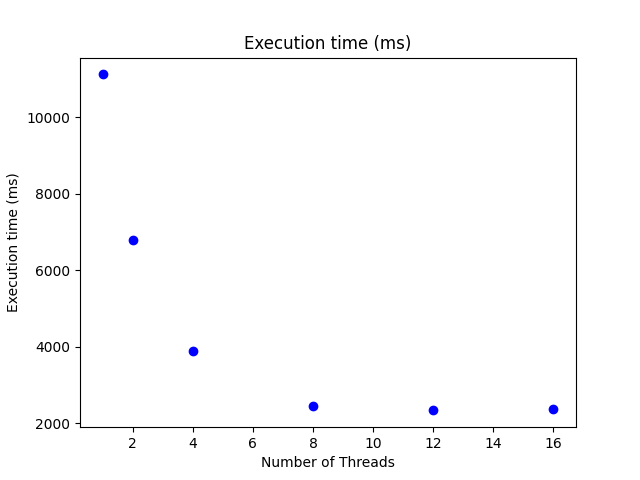
\includegraphics[scale=0.75]{figures/integrate_exe_times.png}}
\caption{Execution time of Riemann integration for different thread counts. Run on a Macbook Pro with 2,2 GHz 6-Core Intel Core i7}
\label{png:integrate}
\end{figure}

The code execution time in \ref{png:integrate} is for the Reimann integral computed with one billion sample values. For one worker thread the execution time was 11.11 seconds. For two threads the execution time was 6.8 seconds, which is nearly double as fast. However as the number of threads increases the increase in execution speed tapers off. Going from 8 to 12 cores only yields a marginal increase in execution speed going from 2.45 second to 2.39. Once more than twelve worker threads are exceeded, there is no longer a marginal increase in speedup. This can be attributed to the physical limitation of threads on the hardware the code was exectuted on. The number of logical cores on the computer that executed this code was 12, meaning that any additional web worker launched after the initial 12 must wait on the thread pool for another to finish before it can be activated. In which case the overhead of launching it is only detrimental to the complete execution time of the program


\subsection{Shared Memory and Atomics}

Web workers with message passing have some similarities in how parallelism is executed with the Erlang programming language. Both of which use message passing to coordinate parallel execution. However many other programming languages and libraries also support and utilize shared memory. An example of this is C/C++ and POSIX threads. Shared memory maps closely to modern multicore hardware, and is faster for certain workloads (TODO GIVE EXAMPLE). However it comes at the cost of a new set of bugs in the shape of data races, which is why languages such as Erlang and Futhark itself abstracts the construct away from the programmer.


JavaScript also offers shared memory through SharedArrayBuffers. A SharedArrayBuffer points to a piece of linear memory. The SharedArrayBuffer can be passed to multiple web workers who can access the memory in parallel. 

In principle safe access to shared memory can be coordinated with message passing, but it's far more efficient for fine grained synchronization to use atomic operations, which again map efficiently to the underlying hardware. Atomic operations make sure that predictable values are written and read, that operations are finished before the next operation starts and that operations are not interrupted (TODO cite Atomics Javascript page). The Atomics package in JavaScript contains functions for performing atomic operations on SharedArrayBuffers. The Atomics package also includes wait and notify functions, like linux futex wait and wake.

To illustrate shared memory and atomics the following example is an implementation of prefix sum. It is a fundamental parallel algorithm which is used as a building block for many other parallel algorithms. The example implements the shared memory 2 pass algorithm from (TODO). 
\begin{listing}[H]    
        \inputminted[fontsize=\small,baselinestretch=0.5,linenos]{javascript}{code/shared/main.js}
        \caption{Main file that calls workers which compute prefix sum using shared memory and atomics in parallel}    
        \label{lst:main-js}    
\end{listing}    

The code in Listing \ref{lst:main-js} spawns 9 worker threads. It sends a message to each of the threads with parameters, some of which are shared array buffers. This allows each of the threads to have access to shared memory. When each thread has sent a message to indicate completion, the final result of prefix sum is logged to the console.

%\captionof{listing}{Example of a worker working}
\begin{listing}[H]    
\inputminted[fontsize=\small,baselinestretch=0.5,linenos]{javascript}{code/shared/prefix_sum.js}
        \caption{Worker file for computing the prefix sum using shared memory and atomics.}    
        \label{lst:prefixsum-js}    
\end{listing}    


The code in Listing \ref{lst:prefixsum-js} handles the actual execution of prefix sum. In the first pass of the algorithm, each thread calculates the prefix sum of their partition in the array, by calling the function prefix\_sum\_partition. Each thread signals that they are done with their work in the first pass by using the Atomics add, and notify functions. The first thread detects signal has accumulated a response of num\_workers - 1, by using the Atomics function wait. At this point the the first thread calculates the cumulative sums of partitions. At this stage it notifies the other other threads using the Atomics store and notify. At this stage all threads calculate the final prefix\_sum, using the precomputed values. On completion each thread sends a message back to the the main file using the postMessage to indicate they are done. 


%TODO: Show speed up over one worker vs 9 workers

%TODO update code to be cleaner and easier to explain

\subsection{Threaded WebAssembly}
There is a proposal to extend the WASM specification with support for threads, namely by leveraging web workers, shared memory, and atomics. Chrome and Firefox and Node.js all have experimental support for threaded WASM. Emscripten supports compilation of C/C++ with pthreads to threaded WASM.

Threaded WASM uses web workers to create and join threads. It doesn't natively invoke web workers but instead handles this by calling out to JavaScript. Shared memory is accomplished by integrating SharedArrayBuffer with WASM's paged memory model. WASM is extended with atomic operation instructions. Putting it concisely the additions of supporting shared array buffers in WASM and adding atomic operations in WASM was all that was needed to facilitate threaded WASM.

A key observation is that WASM does not natively allow for spawning of threads. This is actually taken care of by the runtime or compiler. Specifically for Emscripten, compiling C code written with pthreads will generate three files. It will generate a WASM file, and and two Javascript files. One for the main glue code and other for worker glue code. The glue code takes care of loading the WASM module, populating the memory with the required values, and integrating with the host system as the C code would expect. The C function pthread\_create is translated to Javascript and not WASM. It launches a Javascript Worker, passing it a shared array buffer and the wasm module that it should run. The WASM simply needs the shared array buffer and atomics to synchronize.  

\begin{figure}[htbp]
\centerline{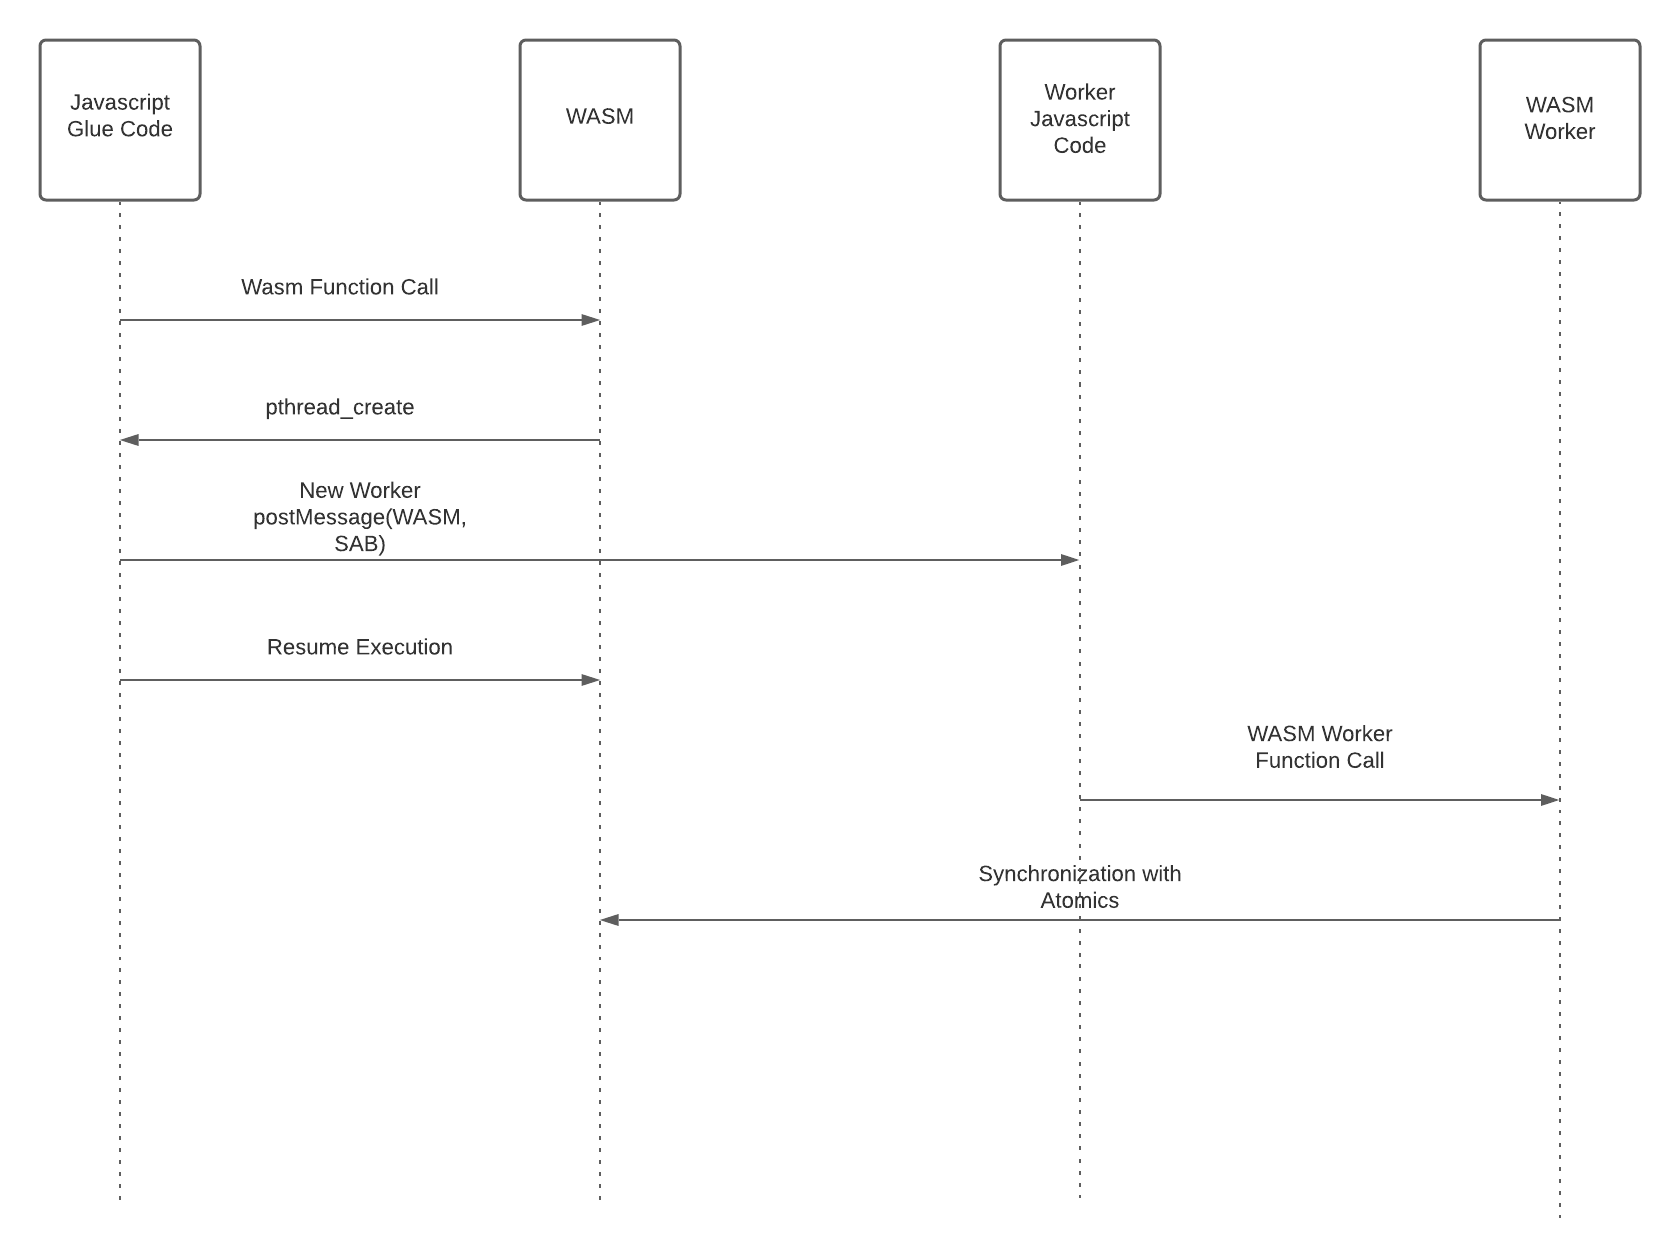
\includegraphics[scale=0.5]{figures/UML_threaded_wasm.png}}
\caption{UML diagram showing flow of execution of threaded programs in WASM}
\label{uml}
\end{figure}

%TODO make updates to UML as specified on piece of paper.

The UML diagram in figure \ref{uml} demonstrates the execution flow of a parallel function written with pthreads in C, compiled by Emscripten, and run in Javascript and WASM. The javascript glue code calls the parallel WASM function, which then calls an external Javascript function that is used to emulate the functionality of pthread\_create. This function launches a new worker, sending it a message with the WASM module, and a shared array buffer, and resumes execution. This JavaScript worker code then  instantiates the WASM module, calling the designated WASM module function. And then with these multiple WASM modules running in parallel, they use atomic instructions native to WASM to facilitate synchronization, as specified in the program.

%TODO: Pthreads + memory growth talk about this

%TODO: Talk about specifying number of web workers up front with Emscripten

%TODO Explain why threaded WASM has no drawbacks becuase it uses the same facilites as javascript for parralel programming while having the speed up of WASM over JS. (Possibly look at over head of launching/loading WASM in a JS worker file).

\newpage

\section{WASM Multicore Backend}
The benchmarks in this section compares Tensorflow and Futhark performance on the
two networks used in the accuracy test, but the benchmark only include the training part of the program

This chapter details the extensions that are added to the Futhark compiler to support a multicore WASM backend. It also benchmarks the generated WASM-multicore code against the sequential WASM backend. It also compares the multicore C backend against the WASM-multicore backend running in the browser.

Fortunately only small adaptions had to be made to the WASM backend developed earlier, to get it running with Multicore. The futhark Compiler has a backend that generates both Sequential C code as well as a backend that generates multicore C code using POSIX threads. As discussed Emscripten can translate multicore C code that uses POSIX threads to multicore WASM that can run in parallel in the browser. The JavaScript API developed in chapter 4 stays unchanged for the WASM-multicore backend. 

Though this thesis adds 2 backends to the 6 backends already present in the Futhark compiler (4 C backends, and 2 Python backends), the added complexity is relatively modest because of the high degree of reuse of code between the two WASM backends. 


\subsection{Implementation Structure}

Below we discuss how to add a new futhark backend that can be invoked from the command line with \texttt{futhark wasm-multicore}. It is structured very similarly to the plain wasm backend described chapter 2. Instead of calling Emscripten on the Sequential C, we apply it to futhark's multicore C backend. We utilize the wasm runtime code written in chapter 2, for the backend and add the necessary Emscripten compiler flags required to enable Multicore WASM. Figure (TBD) illustrates the structure of the WASM multicore implementation.

\begin{figure}[htbp]
\centerline{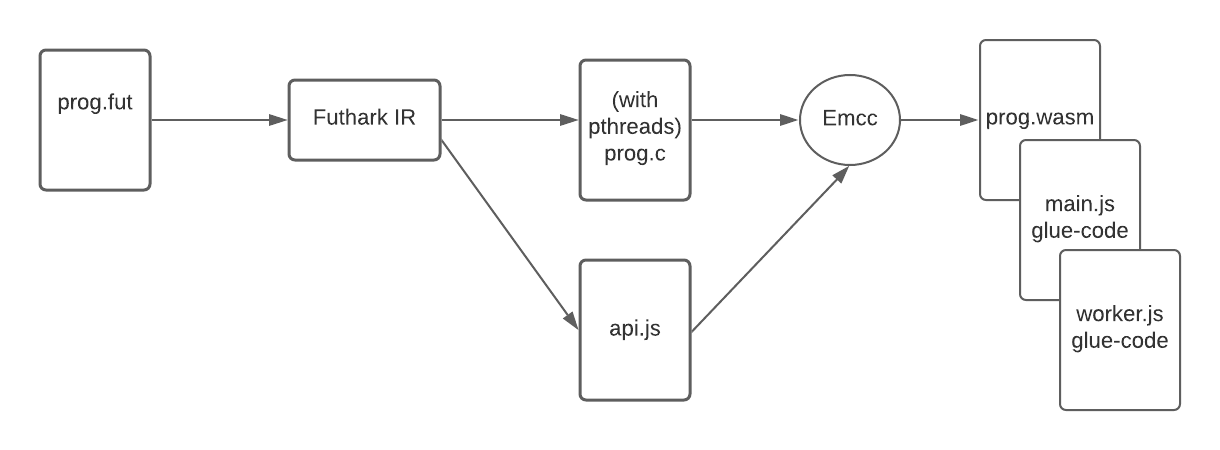
\includegraphics[scale=0.8]{figures/WASM_MC_compiler.png}}
\caption{WASM-multicore compilation}
\label{fig:wasm-mc}
\end{figure}
One of the key differences that can be seen in the figure \ref{fig:wasm-mc} is that the wasm-multicore backend produces 2 JavaScript files and 1 WASM file as opposed to the Sequential Wasm backend which generates 1 JavaScript file and 1 WASM file. The second JavaScript file is the web worker glue code.

\subsection{Implementation Details}
Here we discuss the series of steps that were needed complete the implementation.
\subsubsection{Actions}

The function \textit{compileMulticoreToWASMAction} contains the plumbing for going from futhark source code to WASM and JavaScript glue code. First it calls \textit{MulticoreWASM.compileProg}. This function take the Futhark source code, and runs the multicore C compiler on the source code, as well as generating the Javascript API code.

\textit{MulticoreWASM.compileProg} simply combines the multicore C compiler with the JavaScript code generation discussed in chapter 4, by calling the respective functions that contain the meat of the logic, which have already been developed. The last thing of note is that the flag \textit{-pthread} is passed to \textit{runEMCC}. This flag lets Emcc know that our C code contains pthreads, and thereby compiles it correctly.


\begin{listing}[H]    
        \inputminted[fontsize=\small,baselinestretch=0.5,linenos]{haskell}{code/actionmc.hs}
        \caption{Main file that calls workers which compute prefix sum using shared memory and atomics in parallel}    
        \label{lst:action-mc}    
\end{listing}    
\subsubsection{Multicore C code changes}
The pthread C code generated by the multicore C backend used platform specific implementations in the generated function \textit{getrusage\_thread} and \textit{num\_processors}. For \textit{getrusage\_thread} it was possible to reuse the linux implementation. For \textit{num\_processors} it was necessary to add an additional implementation for the Emscripten platform. This was simply done by including \textit{emscripten/threading.h} and calling the function \textit{emscripten\_num\_logical\_cores}.




\subsubsection{Emscripten Invocation}

The generated multicore C code uses the POSIX function \textit{pthread\_create}. Emscripten aims to follow the POSIX standard closely, but in some places has slightly different behaviour. This is the case for \textit{pthread\_create}, which is a function that is used in the generated multicore C code. 

When pthread\_create() is called, if we need to create a new Web Worker, then that requires returning the main event loop. That is, you cannot call pthread\_create and then keep running code synchronously that expects the worker to start running - it will only run after you return to the event loop (TODO cite pthread docs). In order to work around the API differences, the compiler flag \textit{PTHREAD\_POOL\_SIZE=<integer} needs to be passed to the Emscripten compiler. This effectively creates the web workers before the main thread is called, in which case create\_pthread can just use an already spawned web worker. From testing, this parameter is best set to the number of logical\_cores of the underlying hardware.



\subsubsection{Running in browser with HTTP}



\subsection{Benchmark}






\section{Conclusion}

\end{document}
